\documentclass[12pt]{report}
\usepackage[margin=0.9in]{geometry} % Adjusts the margins
\usepackage{amsmath}
\usepackage{amssymb}
\usepackage[utf8]{inputenc}
\usepackage{noto} % Noto font
\usepackage[dvipsnames]{xcolor} % Allows the use of more colors
\usepackage{titlesec} % Allows customization of titles
\usepackage{tocloft} % Allows customization of the table of contents
\usepackage{hyperref}
\usepackage{graphicx}
\usepackage{placeins}
\usepackage{listings}
% Define the color for the sections
\definecolor{DarkBlue}{RGB}{0,0,239}
\definecolor{DarkerBlue}{RGB}{0,0,150}
\definecolor{DarkestBlue}{RGB}{0,0,42}

% Customize the section titles
\titleformat{\chapter}[display]
  {\normalfont\huge\bfseries\color{DarkBlue}}{\chaptertitlename\ \thechapter}{20pt}{\Huge}
\titleformat{\section}
  {\normalfont\Large\bfseries\color{DarkerBlue}}{\thesection}{1em}{}
\titleformat{\subsection}
  {\normalfont\large\bfseries\color{DarkestBlue}}{\thesubsection}{1em}{}

% Customize the table of contents
\renewcommand{\cftchapfont}{\normalfont\bfseries\color{DarkBlue}}
\renewcommand{\cftsecfont}{\normalfont\color{DarkBlue}}
\renewcommand{\cftsubsecfont}{\normalfont\color{DarkBlue}}
\renewcommand{\cftchappagefont}{\normalfont\bfseries\color{DarkBlue}}
\renewcommand{\cftsecpagefont}{\normalfont\color{DarkBlue}}
\renewcommand{\cftsubsecpagefont}{\normalfont\color{DarkBlue}}

\title{Adaptive Cruise Control System Model}
\author{Your Name}
\date{\today}

\begin{document}


\maketitle
\setcounter{tocdepth}{3}
\tableofcontents


\chapter{Part 1 (a)}
\section{Introduction}
This part presents the derivation of a system model for an Adaptive Cruise Control (ACC) system. The model is based on the longitudinal dynamics of a vehicle and the dynamics of vehicle actuation. The model also considers the travel resistance which includes air drag, rolling resistance, acceleration resistance, and grading resistance.

\section{Vehicle Dynamics Model}
The longitudinal dynamics of a host vehicle is given by the equation:
\begin{equation}
    m\dot{v}_h = m a_f - r_{travel}
\end{equation}
where \(m\) is the vehicle mass, \(v_h\) is the vehicle speed, \(a_f\) is the traction force converted to acceleration, and \(r_{travel}\) is the travel resistance.

The dynamics of a vehicle actuation including engine, transmission, or brake has nonlinear characteristics. The input/output relationship of the actuation dynamics is described as an ordinary differential equation:
\begin{align}
    \dot{x}_f & = f_{act}(x_f, u) \\
    a_f       & = h_{act}(x_f)
\end{align}
where \(x_f \in \mathbb{R}^{n_f}\), \(u \in \mathbb{R}\) are respectively the state, the input of the actuation system. \(u\) is an acceleration command, i.e., a control input calculated by adaptive cruise controller. The output of the system is \(a_f\).

The travel resistance \(r_{travel}\) contains several factors to resist its motion. A model of the resistive force is expressed as
\begin{equation}
    r_{travel} = r_{air} v_h^2 + r_{roll}(v_h) + r_{accel} \dot{v}_h + r_{grad}(\theta)
\end{equation}

\section{State-Space Model for ACC System}
To build a plant model for the ACC system design, two state variables are defined: inter-vehicle distance following error \(\Delta d = d - d_r\) and velocity following error \(\Delta v = v_p - v_h\). The \(d_r\) is determined based on the constant time headway policy given by
\begin{equation}
    d_r = T_{hw}v_h + d_0
\end{equation}
where \(T_{hw}\) is the constant time headway and \(d_0\) is the stopping distance for safety margin.

Let us define the state variables of the plant as \(x = [x_1 \quad x_2 \quad x_3^T]^T \in \mathbb{R}^{2+n_f}\) with \(x_1 = \Delta d\), \(x_2 = \Delta v\) and \(x_3 = x_f\). Then, the state-space model is formulated as
\begin{align}
    \dot{x} & = f(x, u) + Gv + Hw \\
    y       & = Cx + Jv
\end{align}
where
\begin{align*}
    f(x, u) & = \begin{bmatrix}
                    x_2 - T_{hw}x_3 \\
                    -h_{act}(x_f)   \\
                    f_{act}(x_f, u)
                \end{bmatrix}, \\
    G       & = \begin{bmatrix}
                    T_{hw}/m \\
                    1/m      \\
                    0
                \end{bmatrix},           \\
    H       & = \begin{bmatrix}
                    0 \\
                    1 \\
                    0
                \end{bmatrix},           \\
    C       & = \begin{bmatrix}
                    1 & 0 & 0 \\
                    0 & 1 & 0 \\
                    0 & 0 & 1
                \end{bmatrix},           \\
    J       & = \begin{bmatrix}
                    0 \\
                    0 \\
                    -1/m
                \end{bmatrix}
\end{align*}
where \(u \in \mathbb{R}\) and \(y = [\Delta d \quad \Delta v \quad \dot{v}_h]^T \in \mathbb{R}^3\) are the input and output of the plant and \(v = r_{travel}\) and \(w = \dot{v}_p\) represents disturbances into the plant.

\section{SS Model Representation}

The plant model for MPC is simplified to reduce computational cost. The actuation system model is approximated to a switched linear time variant system as follows:

\begin{equation}
\begin{aligned}
\dot{x}_f &= A_f(t)x_f + B_f(t)u \\
a_f &= C_fx_f
\end{aligned}
\end{equation}

where \(x_f \in \mathbb{R}\), \(n_f = 1\), and

\[
A_f(t) = 
\begin{cases} 
-1/T_{eng}, & \text{if } u(t) \geq a_{thr_{off}} \\
-1/T_{brk}, & \text{if } u(t) < a_{thr_{off}}
\end{cases}
\]

\[
B_f(t) = 
\begin{cases} 
K_{eng}(t)/T_{eng}, & \text{if } u(t) \geq a_{thr_{off}} \\
K_{brk}(t)/T_{brk}, & \text{if } u(t) < a_{thr_{off}}
\end{cases}
\]

and \(C_f = 1\).

The steady-state gains can be changed to compensate the prediction accuracy. For example, \(K_{eng}(t)\) is composed of constant value \(K_c\) and compensation signal \(\Delta K(t)\) as below.

\begin{equation}
K_{eng}(t) = K_c + \Delta K(t)
\end{equation}

where \(\Delta K(t)\) is computed by the filter \(\Delta K(s) = L(s)u(s)\) with \(L(0) = 0\). 

The prediction model can be simplified to the linear time variant system with three states below:

\begin{equation}
\begin{aligned}
\dot{x} &= A(t)x + B(t)u + Gv + Hw \\
y &= Cx + Jv
\end{aligned}
\end{equation}

where \(x \in \mathbb{R}^3\) and

\[
A(t) = 
\begin{bmatrix}
0 & 1 & -T_{hw} \\
0 & 0 & -1 \\
0 & 0 & A_f(t)
\end{bmatrix}, 
B(t) = 
\begin{bmatrix}
0 \\
0 \\
B_f(t)
\end{bmatrix}
\]

The travel disturbance model can be written as

\begin{equation}
r_{travel} = r_{accel} \dot{v}_h + r_{travel}
\end{equation}

where the first term is the acceleration resistance and the second term is other resistances \(r_{travel} = r_{air} v_h^2 + r_{roll}(v_h) + r_{grad}(\theta)\).

Let us define a state transformation for \(x_3\) as below.

\begin{equation}
\tilde{x}_3 = \frac{1}{1 + r_{accel}/m} x_3
\end{equation}

From the vehicle dynamics, the acceleration of the host vehicle becomes

\begin{equation}
\dot{v}_h = x_3 - \frac{1}{m} r_{travel} = (1 + r_{accel}/m) \tilde{x}_3 - \frac{1}{m}
_{travel}
\end{equation}

Substituting this into the travel disturbance model gives

\begin{equation}
r_{travel} = r_{accel} \tilde{x}_3 + \frac{1}{1 + r_{accel}/m} r_{travel}^2
\end{equation}

The travel resistance can be described using the new state \(\tilde{x}_3\) instead of \(\dot{v}_h\). Finally, the state transformation and the travel disturbance model yield the prediction model with the new state coordination below:

\begin{equation}
\begin{aligned}
\dot{x} &= A(t)x + B(t)u + Gv + Hw \\
y &= Cx + Jv
\end{aligned}
\end{equation}

where

\[
x = [\Delta d, \Delta v, \rho_{accel}x_f]^T \in \mathbb{R}^3, \quad v = r_{travel}, \quad w = \dot{v}_p
\]

and

\[
A(t) = 
\begin{bmatrix}
0 & 1 & -T_{hw} \\
0 & 0 & -1 \\
0 & 0 & A_f(t)
\end{bmatrix}, 
B(t) = 
\begin{bmatrix}
0 \\
0 \\
\rho_{accel}B_f(t)
\end{bmatrix}
\]

\[
G = 
\begin{bmatrix}
\rho_{accel}T_{hw}/m \\
\rho_{accel}/m \\
0
\end{bmatrix}, 
H = 
\begin{bmatrix}
0 \\
1 \\
0
\end{bmatrix}
\]

\[
C = 
\begin{bmatrix}
1 & 0 & 0 \\
0 & 1 & 0 \\
0 & 0 & 1
\end{bmatrix}, 
J = 
\begin{bmatrix}
0 \\
0 \\
-\rho_{accel}/m
\end{bmatrix}
\]

\[
\rho_{accel} = \frac{1}{1 + r_{accel}/m}
\]

\chapter{Suitability of MPC for the Control Problem}

Model Predictive Control (MPC) is particularly suitable for solving the control problem due to several key features of the system:

\section{Time-Varying Dynamics}
The system dynamics are time-varying, which can be handled effectively by MPC because it uses a model of the system to predict future behavior.

\section{Presence of Disturbances}
The system is subject to disturbances, such as travel disturbance. MPC can account for these in its predictions and adjust control actions accordingly.

\section{Constraints}
The system has constraints on both the control inputs and the system states. MPC is well-suited to handle such constraints.

\section{Need for Optimization}
The system requires an optimization of a cost function, which could be related to energy consumption, system performance, etc. MPC operates by solving an optimization problem at each time step.

\section{Requirement for Adaptability}
The system parameters or dynamics can change over time. MPC can adapt to these changes by updating the prediction model at each sampling time.

\section*{Result}
These features make MPC a powerful and flexible control strategy that can handle complex control problems in a systematic and efficient manner.

\chapter{Controller Design Formulation}

\section{Cost Matrices}
In our Model Predictive Control (MPC) setup, we define the cost matrices $\mathbf{Q_t} = I$, $\mathbf{R_{t_{\Delta u}}} = I$, and $\mathbf{R_{t_u}} = I$, where $I$ represents the identity matrix. 

These matrices respectively penalize the tracking error, the rate of change, and the magnitude of the control input. We then iteratively adjust these matrices to optimize the system performance. Higher weights on the tracking error ($w_{y1}(t)$) or on the control input's change rate ($w_{\Delta u}(t)$) result in a more aggressive controller or smoother control inputs, respectively.


\section{Constraints}
In the MPC formulation, we apply constraints based on the physical limitations of the system. These constraints, which involve the control input \(u\), its increment \(\Delta u\), and the output \(y\), are all subject to upper and lower bounds, as represented by the "min" and "max" suffixes. The specific values for these limits are determined by the actuation system's capabilities and the desired operational range of the system. We set the following requirements as constraints:

\begin{enumerate}
    \item The relative velocity must not be excessively large, unless a preceding vehicle is initially detected outside of the range.
    \item The acceleration of the host vehicle must be greater than or equal to -0.25 [G].
    \item The acceleration change must be gradual, with the exception of traffic jam scenarios.
\end{enumerate}

These requirements are carefully integrated into the MPC formulation to ensure the system operates within safe and efficient parameters.


\section{Disturbances}
The system is subject to disturbances, such as travel disturbance. These disturbances can cause prediction errors and degrade control performance. In the MPC formulation, the effect of these disturbances is explicitly considered in the prediction model. This allows the controller to compensate for the disturbances and maintain good performance. The specific effect of the disturbances on the feedback loop depends on their magnitude and frequency, and can be studied through simulation or experimental testing.

\section{Dual Mode Prediction}
The control input \(u(t)\) guides the selection of the appropriate model, thereby creating a dual model system. Here are the matrices \(A(t)\) and \(B(t)\) for the two different cases:

\[
\begin{aligned}
&A_{eng}(t) = 
\begin{bmatrix}
0 & 1 & -T_{hw} \\
0 & 0 & -1 \\
0 & 0 & -1/T_{eng}
\end{bmatrix}, 
&B_{eng}(t) = 
\begin{bmatrix}
0 \\
0 \\
K_{eng}(t)/T_{eng}
\end{bmatrix}, 
\end{aligned}
\]

\[
\begin{aligned}
&A_{brk}(t) = 
\begin{bmatrix}
0 & 1 & -T_{hw} \\
0 & 0 & -1 \\
0 & 0 & -1/T_{brk}
\end{bmatrix}, 
&B_{brk}(t) = 
\begin{bmatrix}
0 \\
0 \\
K_{brk}(t)/T_{brk}
\end{bmatrix},
\end{aligned}
\]

If \(u(t) \geq a_{thr_{off}}\), we use the \(A_{eng}(t)\) and \(B_{eng}(t)\) matrices, which reflect the engine dynamics. Conversely, if \(u(t) < a_{thr_{off}}\), we switch to the \(A_{brk}(t)\) and \(B_{brk}(t)\) matrices, which encapsulate the brake dynamics. This dual model system allows the controller to adapt to the changing conditions of the vehicle's operation.

\begin{lstlisting}[language=Matlab]
    % Your system
    A = [0 1 -1.3; 0 0 -1; 0 0 -2.17];
    B = [0; 0; -1.5];
    Q = eye(3);  
    R = 1;  
    
    % LQR
    K = lqr(A, B, Q, R);
    
    % Check stability by checking eigenvalues of (A-BK)
    eig_A_BK = eig(A - B*K);
    if all(real(eig_A_BK) < 0)
        disp('The system is asymptotically stable.')
    else
        disp('The system is not asymptotically stable.')
    end

    >>> The system is asymptotically stable.
    \end{lstlisting}
\begin{figure}
    \centering
    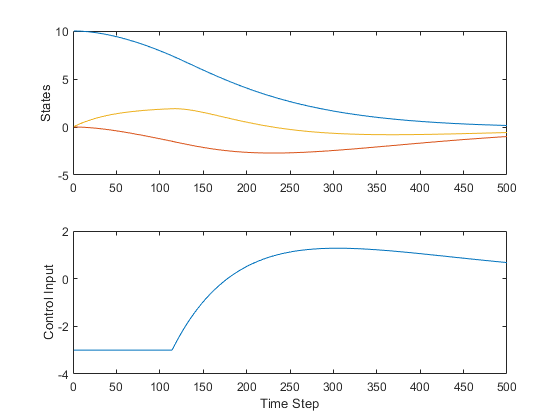
\includegraphics[width = 0.8 \textwidth]{untitled.png}
    \caption{Behaviour when distance is relatively big}
\end{figure}

\begin{figure}
    \centering
    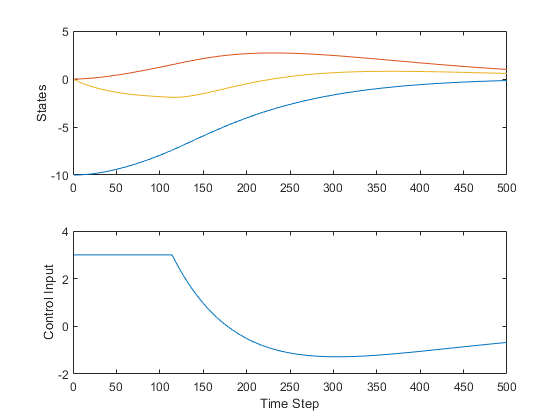
\includegraphics[width = 0.8 \textwidth]{geride.png}
    \caption{Behaviour when distance is relatively negative}
\end{figure}

\begin{figure}
    \centering
    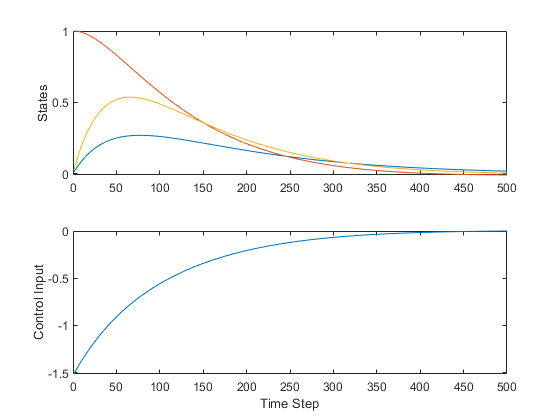
\includegraphics[width = 0.8 \textwidth]{hiz.png}
    \caption{behavior when relative speed is high}
\end{figure}

\begin{figure}
    \centering
    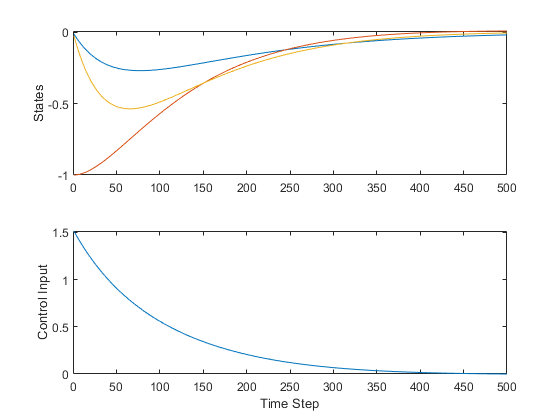
\includegraphics[width = 0.8 \textwidth]{slow.png}
    \caption{behavior when relative speed is slow}
\end{figure}

\begin{figure}
    \centering
    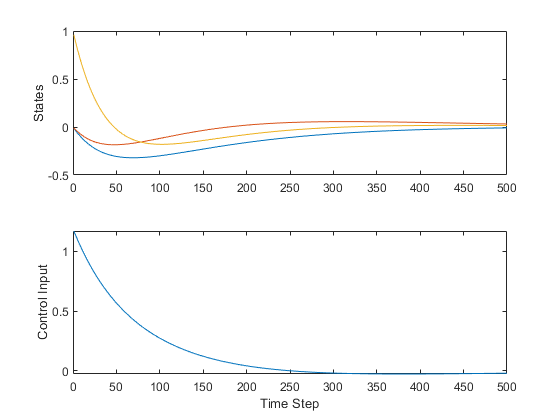
\includegraphics[width = 0.8 \textwidth]{accelerated.png}
    \caption{behaviour when relative acceleration is high}
\end{figure}

\begin{figure}
    \centering
    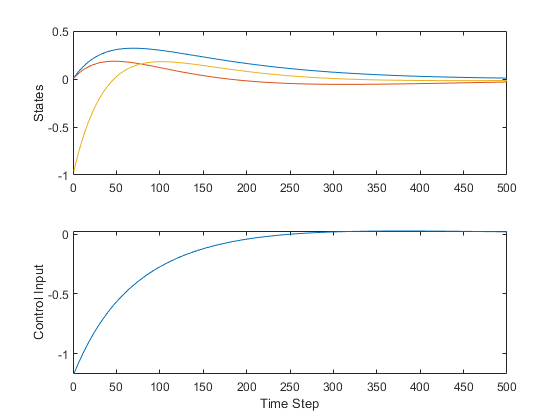
\includegraphics[width = 0.8 \textwidth]{decelereted.png}
    \caption{behaviour when relative acceleration is negative}
\end{figure}

Note: I cannot add chain reaction into matlab.


\chapter{Part 2}


\section{a. Simulink model for Apollo satellite}

All simulations are for 40 seconds starting from $t = 0$.


As can be observed from Figures 4.1 and 4.2, the step size decreases as the velocity of the satellite increases (in fact it is about 4. order derivative term). This enables providing more accurate data with higher resolution in areas where the satellite moves at high speeds. 

The obtained trajectories with a step size of 0.001 are consistent and realistic. However, when we increase the step size to 0.01, the resulting trajectories are inaccurate. In the simulation performed with the Runge-Kutta method and a fixed step size, a successful result is also obtained. 

However, similar to the variable step size case, when the step size increases, we obtain an erroneous simulation with Runge-Kutta as well. Additionally, while the fixed step size simulation was successful, the simulation with fixed step size took approximately 10 times longer. According to internet if system is complicated this speed difference can goes up to 100,000 times. 

Variable step size simulations maintain the accuracy of calculations and improve performance, especially for systems with highly variable velocity and acceleration values.



\begin{figure}
    \centering
    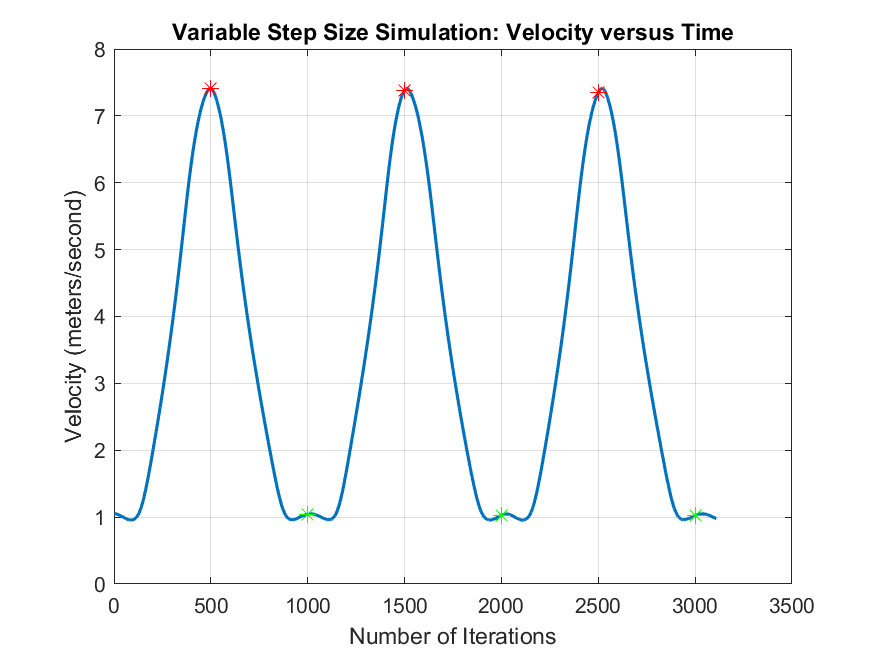
\includegraphics[width = 0.8 \textwidth]{Figure_2.png}
    \caption{Satellite speed}
    \label{fig2}
\end{figure}

\begin{figure}
    \centering
    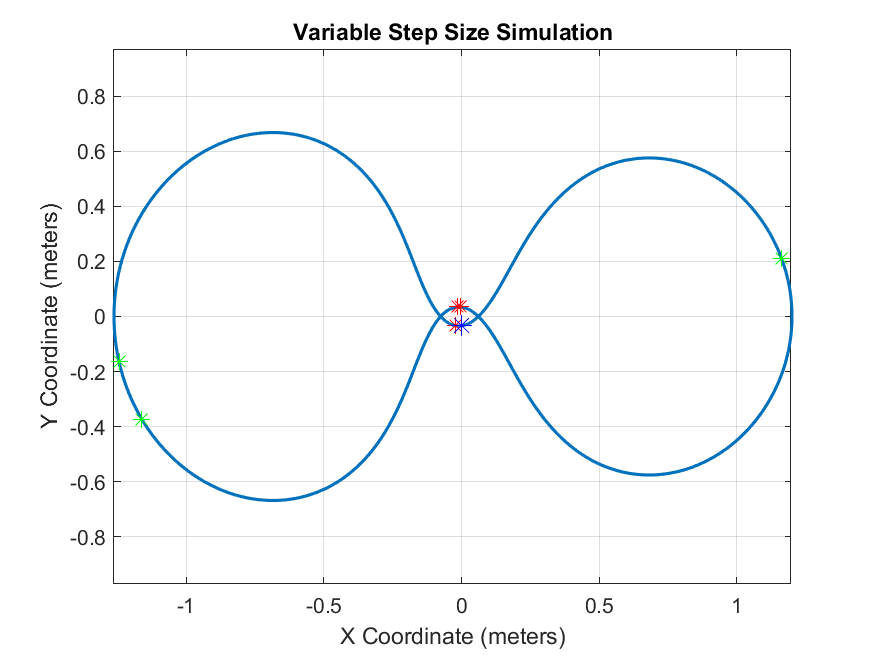
\includegraphics[width = 0.8 \textwidth]{Figure_3.png}
    \caption{Orbit}
\end{figure}




\begin{figure}
    \centering
    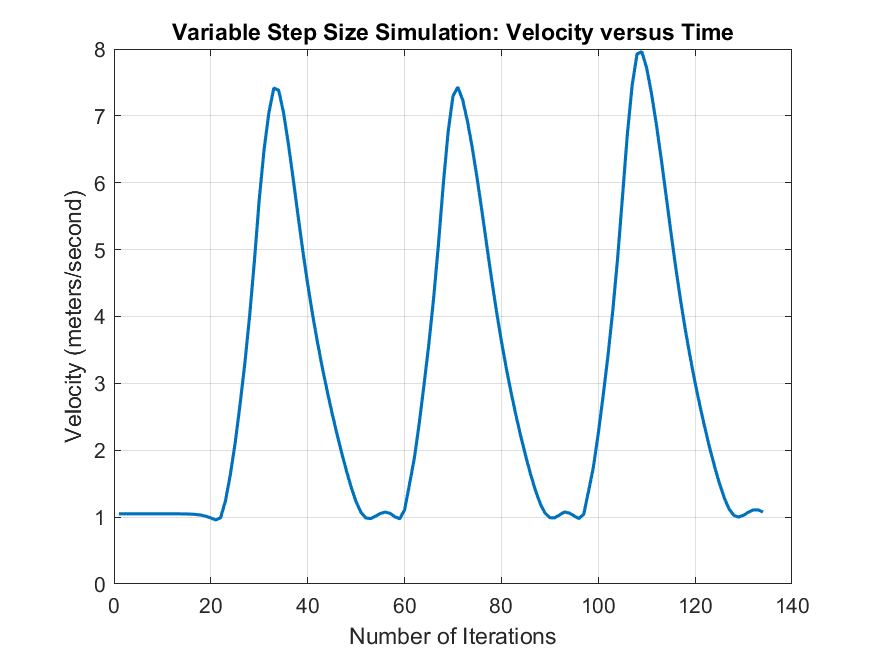
\includegraphics[width = 0.8 \textwidth]{variable (2).png}
    \caption{h = 0.01, variable step size simulation}
\end{figure}
\begin{figure}
    \centering
    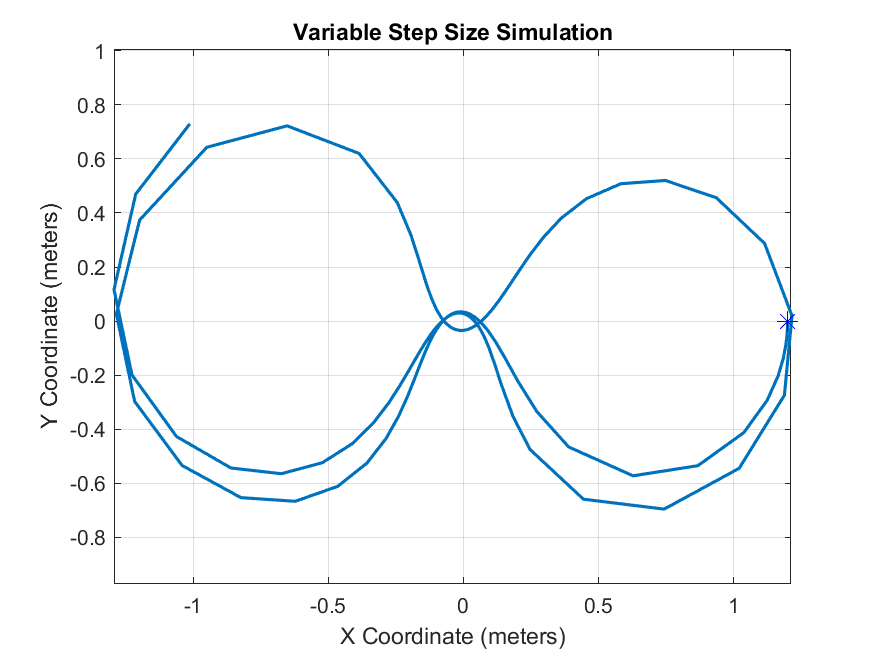
\includegraphics[width = 0.8 \textwidth]{variable (3).png}
    \caption{h = 0.01, variable step size simulation}
\end{figure}

\FloatBarrier

\section{Implementation and Testing of the Runge-Kutta Method}

The Runge-Kutta method is a numerical technique used to solve ordinary differential equations (ODEs). The fourth-order Runge-Kutta method, often simply referred to as the "RK4 method," is commonly used due to its balance between computational efficiency and accuracy. 

\subsection{Method Implementation}

The RK4 method approximates the solution to an ODE by taking a weighted average of four increments, where each increment is the estimated change over a small interval of time (or a 'step'). These increments are calculated at the beginning of the interval, at the midpoint, and at the end. The general formula for the RK4 method is as follows:

\begin{align*}
k_1 &= h \cdot f(t_n, y_n) \\
k_2 &= h \cdot f(t_n + \frac{h}{2}, y_n + \frac{k_1}{2}) \\
k_3 &= h \cdot f(t_n + \frac{h}{2}, y_n + \frac{k_2}{2}) \\
k_4 &= h \cdot f(t_n + h, y_n + k_3) \\
y_{n+1} &= y_n + \frac{1}{6} \cdot (k_1 + 2k_2 + 2k_3 + k_4)
\end{align*}

Where $h$ is the step size, $t_n$ is the current time, $y_n$ is the current value, and $f(t, y)$ is the derivative of $y$.

\subsection{Choosing a Suitable Step Size}

The choice of step size $h$ is crucial for the performance of the RK4 method. A smaller step size will generally result in a more accurate solution, but at the cost of requiring more computational resources. Conversely, a larger step size will be more efficient but less accurate.

A suitable step size can often be determined empirically. 0.001 in this case.

\subsection{Testing the Method}

\begin{figure}
    \centering
    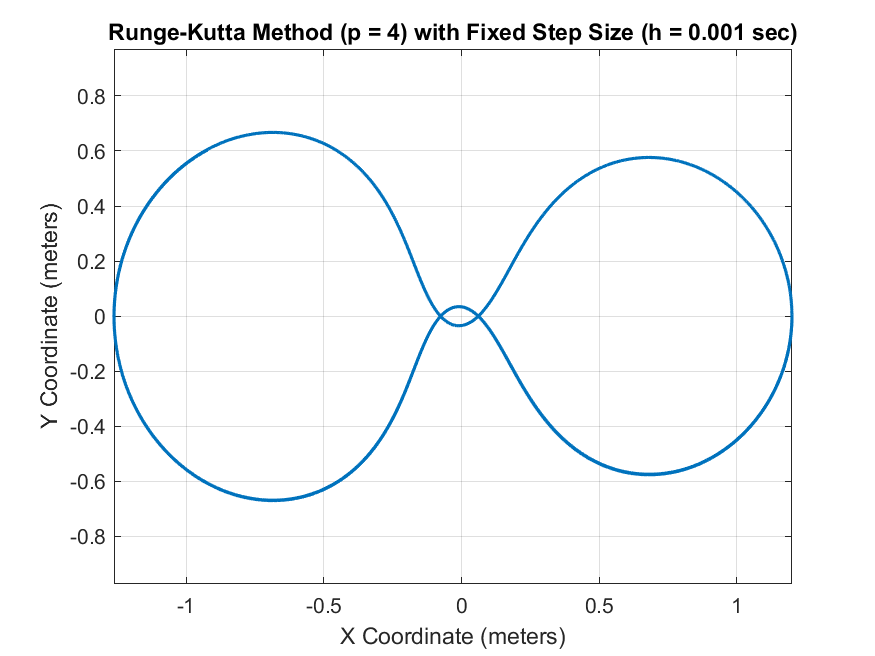
\includegraphics[width = 0.8 \textwidth]{Figure_4.png}
    \caption{Orbit of Runge-Kutta fixed size p = 4, h = 0.001}
\end{figure}

\begin{figure}
    \centering
    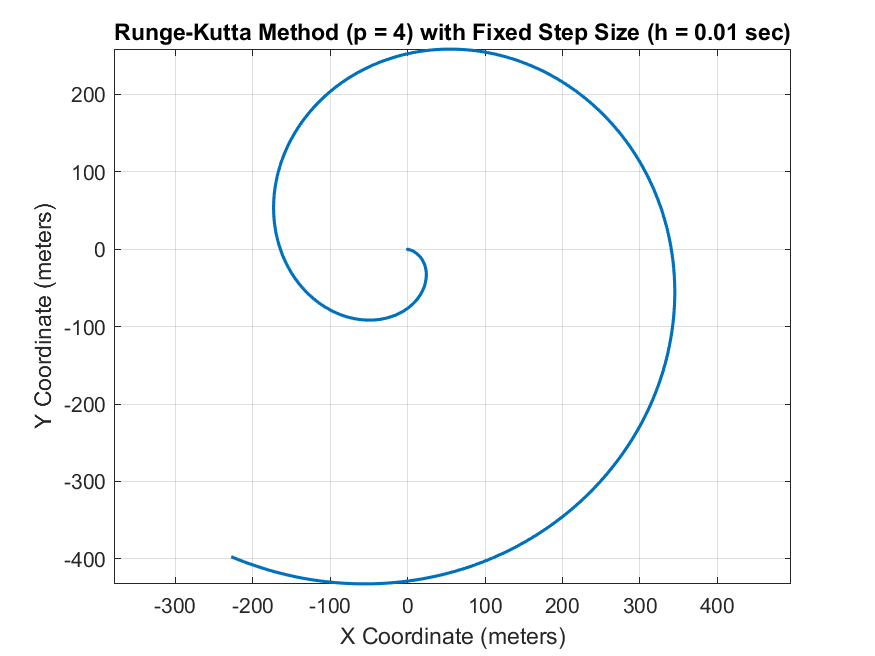
\includegraphics[width = 0.8 \textwidth]{step.png}
    \caption{Orbit of Runge-Kutta fixed size p = 4, h = 0.01}
\end{figure}

\FloatBarrier
\section{Realization of Variable Step Size in Numerical Solvers}

In numerical methods such as the Runge-Kutta for solving ordinary differential equations (ODEs), it's often advantageous to have a variable step size. This approach adjusts the step size dynamically based on the local behavior of the solution, allowing the method to take larger steps when the solution is changing slowly and smaller steps when it's changing rapidly. 

\section{Main Implementation Steps for a Variable Step Size Solver}

\begin{enumerate}
    \item \textbf{Initial Step Size Selection:} Start with a suitable initial step size. This could be a default small value, or it could be estimated based on the problem characteristics or initial error tolerance.

    \item \textbf{Step Size Estimation:} After each step, estimate the local truncation error of the numerical method. This could be done, for instance, by taking a full step and two half steps and comparing the results.

    \item \textbf{Step Size Adjustment:} Adjust the next step size based on the estimated error. If the error is below the tolerance, increase the step size; if it's above the tolerance, decrease the step size.

    \item \textbf{Solution Update:} If the error is below the tolerance, accept the new solution and move to the next step. If it's above the tolerance, reject the step and repeat it with the smaller step size.

    \item \textbf{Repeat:} Repeat steps 2-4 until the solution has been found for all desired values of the independent variable.

    \item \textbf{Post Processing:} After the solution has been found, the step sizes used can be post processed for analysis. This can provide insight into the problem areas where smaller step sizes were needed, or regions where larger step sizes could be used.
\end{enumerate}

\section*{RK4 System with adaptive step size}

\begin{lstlisting}
while t < t_end
    % RK4 step
    k1 = f(t, y);
    k2 = f(t + h/2, y + h/2 * k1);
    k3 = f(t + h/2, y + h/2 * k2);
    k4 = f(t + h, y + h * k3);
    y_new = y + h/6 * (k1 + 2*k2 + 2*k3 + k4);

    % Heun's method for error estimation
    y_star = y + h/2 * (k1 + k4);

    % Estimate error
    err = abs(y_new - y_star);

    % Update step size
    if err < absTol + relTol * abs(y_new)
        % Accept step
        t = t + h;
        y = y_new;
        T = [T, t];
        Y = [Y, y];
        H = [H, h];
        h = h * 1.2;
    else
        % Reject step
        h = h * 0.8;
    end
end
\end{lstlisting}
\FloatBarrier
\begin{figure}
    \centering
    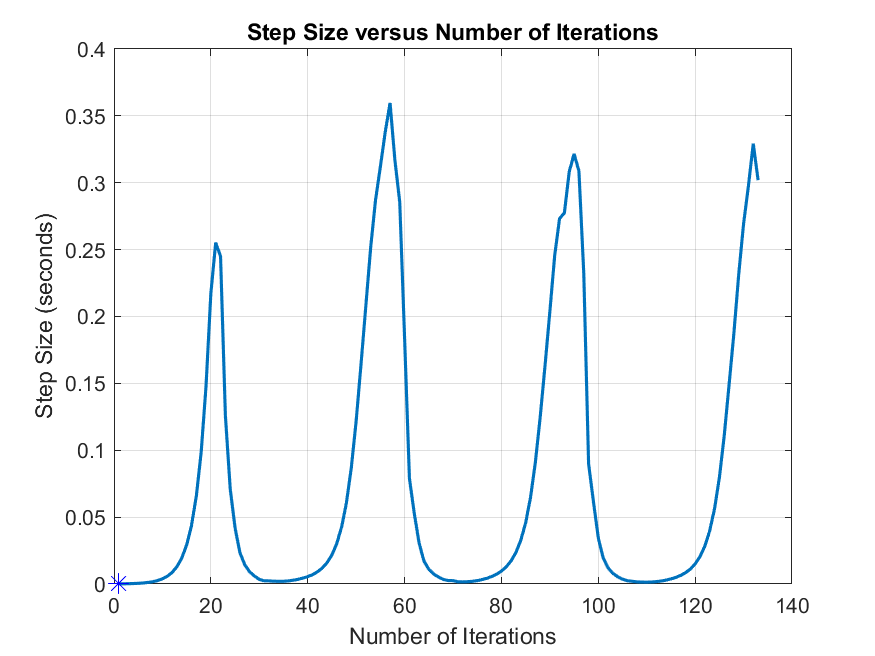
\includegraphics[width = 0.8 \textwidth]{variable (1).png}
    \caption{h = 0.01, variable step size simulation}
\end{figure}

\begin{figure}
    \centering
    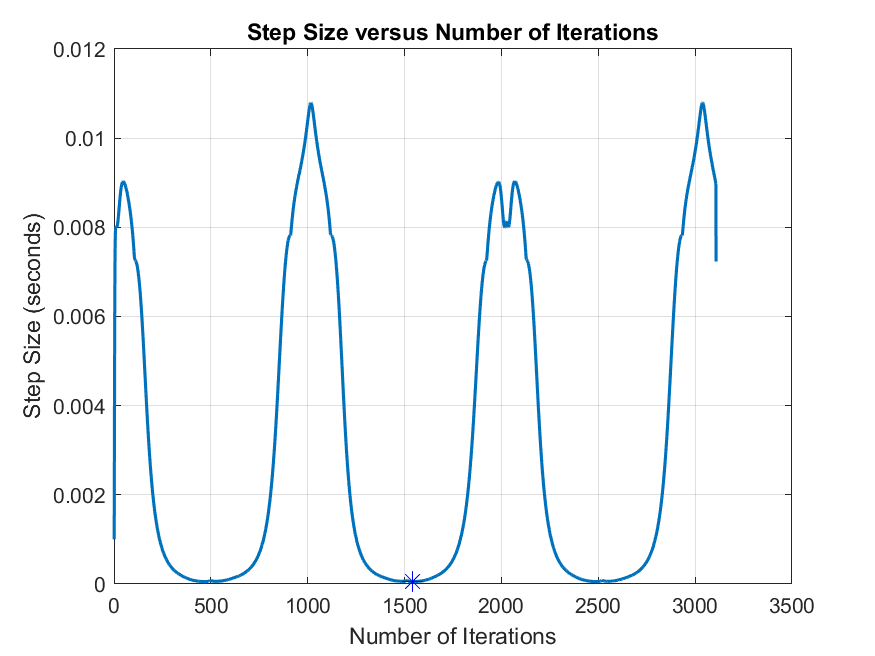
\includegraphics[width = 0.8 \textwidth]{Figure_1.png}
    \caption{h = 0.001, variable step size simulation}
\end{figure}
\FloatBarrier
The changes in the step sizes over the course of the simulation are a reflection of the complexity and non-linearity of the system's dynamics at different points in time.

When we look at the trajectory of the satellite and the associated step sizes, we observe that the step size decreases (i.e., the computation becomes more detailed) during periods when the satellite's trajectory is changing rapidly or in a complex manner. This could include moments when the satellite is making a sharp turn, accelerating rapidly, or passing close to a planet or other massive object that affects its trajectory.

Conversely, when the satellite's trajectory is relatively simple and predictable (for example, when it's moving in a straight line or following a steady curve), the solver might be able to take larger steps, because the error of approximation remains within acceptable bounds even over these longer intervals.

\end{document}
